\chapter{Zwei Zellen: aus Verbindung wird Dynamik}
\label{ch:two}
\begin{bild}{Aktualisierung v1.5: der Übergang zu vielen Zellen ist genauer}
Kapitel~\ref{ch:scaling15} beweist für ganze wachsende Familien, wann die Lücke bestehen bleibt und wann eine ausdrücklich gewählte innere Transferdynamik kritisch wird. Der exakt bekannte 544D-Stern und die größere C16-Zelle werden dabei nicht verwechselt. Lokale statische Stabilität ist noch keine vollständige dynamische Grenzkontrolle.
\end{bild}
\section{Warum die Zellen beim Verbinden ihre Reinheit verlieren}
Ist eine reduzierte Dichtematrix $\rho_A=\ket\Omega\bra\Omega$ rein, so muss der gemeinsame Zustand bezüglich $A$ und seinem Rest faktorisiert sein. Sein Träger liegt in $\C\Omega\otimes\mathcal H_B$. Sind alle disjunkten Zellmarginalien unverändert rein, ist der Gesamtzustand ein Produkt über die Zellen.

Deshalb können gekoppelte Zellen nicht zugleich unverändert reine $\Omega$-Zustände bleiben und miteinander verschränkt sein. Sie können im Produkt beginnen und dann korrelieren. Oder $\Omega$ bezeichnet eine lokale Verknüpfungsamplitude und nicht die physische Dichtematrix jeder Region. Diese Unterscheidung eröffnet einen konsistenten Weg zu größeren Netzen. \src{S03, §2 und §7}

\section{Ein kleiner exakter Raum in einem großen Hilbertraum}
Zwei vollständige Tetramerzellen mit genau einer Brücke haben
\begin{equation}
H=H_A+H_B+\lambda V,\qquad V=(I+S_{ab})/2,\quad J>0,\ \lambda\ge0.
\end{equation}
Der volle Raum besitzt $4^8=65536$ Dimensionen. Trotzdem bleibt die Entwicklung des Produktzustands in einem zweidimensionalen invarianten Unterraum:
\begin{equation}
\ket0=\ket\Omega_A\ket\Omega_B,\qquad
\ket1=\frac{4S_{ab}-I}{\sqrt{15}}\ket0.
\end{equation}
Die beiden Vektoren sind orthonormal; $H_0\ket0=0$ und $H_0\ket1=4J\ket1$. Es folgt
\begin{equation}
\boxed{H_{\mathrm{red}}=
\begin{pmatrix}
5\lambda/8&\sqrt{15}\lambda/8\\
\sqrt{15}\lambda/8&4J+3\lambda/8
\end{pmatrix}.}
\label{eq:Hred}
\end{equation}
Die Brücke koppelt den Produktgrundzustand an eine gemeinsame adjungierte Anregung. Beide Zellhälften verwenden dabei einen bestimmten 15-dimensionalen Unterraum ihrer jeweils 45-dimensionalen ersten Anregungsfläche. \src{S01, §4; S03, §3; hier auf allen 65536 Komponenten exakt geprüft}

\section{Energie und ein wirklicher Grundzustandsnachweis}
Mit
\begin{equation}
R=\sqrt{16J^2-2J\lambda+\lambda^2}
\end{equation}
lauten die beiden Eigenwerte
\begin{equation}
E_\pm=\frac{4J+\lambda\pm R}{2},\qquad
E_-=\frac{5\lambda}{8}-\frac{15\lambda^2}{256J}
-\frac{15\lambda^3}{4096J^2}+O(\lambda^4/J^3).
\end{equation}
Die negative Korrektur beschreibt die Absenkung gegenüber dem einfachen Produktwert $5\lambda/8$.

Ein exakter Eigenzweig ist noch kein globaler Grundzustandsbeweis. Hier gibt es aber eine zusätzliche Schranke: Der zweite Eigenwert von $H_A+H_B$ ist $2J$. Wegen $\lambda V\ge0$ kann der zweite Eigenwert des gekoppelten $H$ nicht darunter fallen. Solange $E_-<2J$, ist der gefundene Eigenwert also der eindeutige globale Grundwert. Das ist genau der Bereich
\begin{equation}
0\le\lambda<8J,\qquad
\Delta_{\mathrm{gap}}\ge2J-E_-=\frac{R-\lambda}{2}>0.
\label{eq:gapbound}
\end{equation}
Bei $\lambda\ge8J$ endet nur dieser historische Nachweis. Version 1.3 kontrolliert die Konkurrenzsektoren für dasselbe Zweizellenmodell nun bei allen endlichen $\lambda\ge0$. Mit $Q=\sqrt{4J^2+\lambda^2}$ gilt
\begin{equation}
E_0=E_-,\quad E_1=3J+\lambda/2-Q/2,\quad
\Delta_{\mathrm{gap}}=J+(R-Q)/2>J/2.
\label{eq:alllambda13}
\end{equation}
Der Grundzustand bleibt eindeutig; $8J$ und $16J/5$ waren Beweisgrenzen, keine Phasenübergänge. Der vollständige Beweis steht in Kapitel~\ref{ch:audit13}. Er gilt für zwei vollständige Tetramer mit einer Brücke, nicht für beliebig große Netze.

\begin{figure}[H]\centering
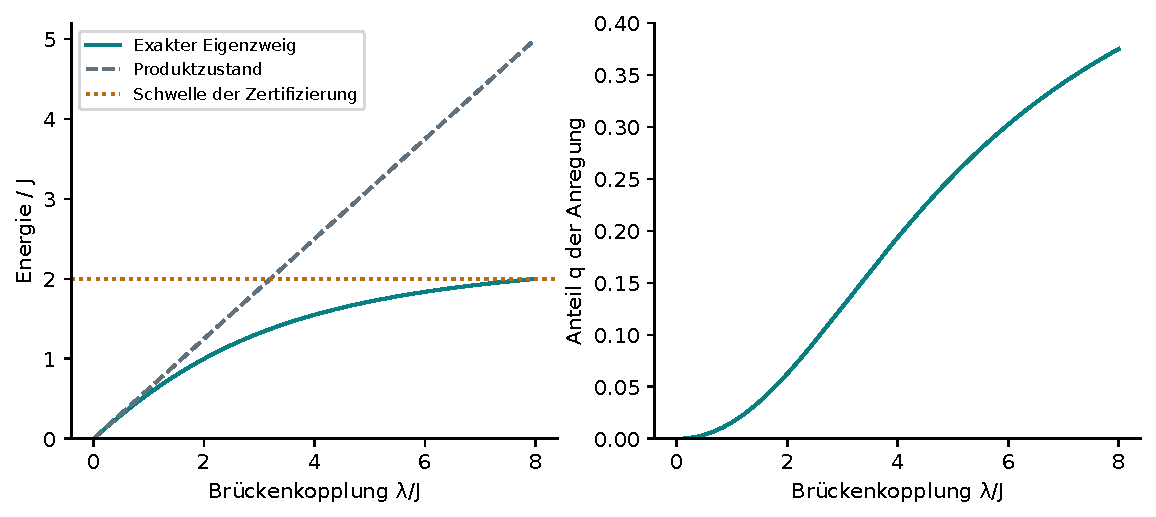
\includegraphics[width=\linewidth]{figures/two_cells.pdf}
\caption{Links der exakte Zweizellen-Eigenzweig und der Produktwert. Die Linie $2J$ illustriert die ältere hinreichende Schranke, nicht die Grenze des neuen allkoppligen Satzes. Rechts der Anregungsanteil $q$. Die Kurven sind berechnete Modellwerte.}
\end{figure}

\begin{center}
\begin{tabular}{rrrr}
\toprule $\lambda/J$&$E_-/J$&Untere Gapgrenze$/J$&Gap nach S08\\\midrule
0&0&2&2\\
0,5&0,29743758&1,70256242&1,922\\
1&0,56350833&1,43649167&1,818\\
2&1&1&1,586\\
3,2&1,37289425&0,62710575&1,340\\
6&1,83772234&0,16227766&1,000\\\bottomrule
\end{tabular}
\end{center}
Die Untergrenze ist nicht der exakte Gap. Die Werte der letzten Spalte sind Quellnumerik. Der ältere Nachweis $\Delta\ge2J-5\lambda/8$ war korrekt, aber schwächer und nur bis $\lambda<16J/5$ positiv.

\section{Verschränkung aus derselben Kopplung}
Der niedrige Eigenzustand lässt sich schreiben als
\begin{equation}
\ket{\Psi_-}=\sqrt{1-q}\ket0-\sqrt q\ket1,
\qquad q=\frac12\left(1-\frac{4J-\lambda/4}{R}\right).
\end{equation}
Seine Zellreduktion besitzt das Spektrum
\begin{equation}
\spec\rho_A=\{1-q,(q/15)^{[15]},0^{[240]}\}.
\end{equation}
Die Entropie in natürlichen Logarithmen ist
\begin{equation}
S_A=-(1-q)\log(1-q)-q\log(q/15).
\end{equation}
Bei $\lambda=J$ sind $q\approx0{,}0158771$ und $S_A\approx0{,}1245231$; bei $\lambda=2J$ gilt $q=1/16$. Schon eine endliche einzelne Brücke macht die lokale Zelle gemischt. Energieabsenkung und Verschränkung sind hier keine unabhängig eingesetzten Zusätze.

Die isolierten Reduktionen von $\Omega$ sind hingegen
\begin{equation}
\rho_k=\frac{P_{\Lambda^k\C^4}}{\binom4k},\qquad k=1,2,3.
\end{equation}
Auf ihrem Träger ist $-\log\rho_k$ skalar. Ihr endlicher modularer Fluss ist dort trivial. Im gekoppelten Zustand entsteht eine modulare Wertdifferenz $\log[15(1-q)/q]$. Sie ist dimensionslos und noch keine physikalische Zeit. Nullräume dürfen dabei nicht mit einem undefinierten Logarithmus behandelt werden. \src{S03, §4 und §6}

\section{Ein Uhrsignal ohne zusätzlich gewählten lokalen Tick}
Starte im Produkt $\ket0$ und lasse denselben konstanten gekoppelten Hamiltonoperator wirken. Dann gilt
\begin{equation}
p_1(t)=\frac{15\lambda^2}{16R^2}\sin^2\left(\frac{Rt}{2\hbar}\right),
\qquad \langle H_A+H_B\rangle_t=4Jp_1(t).
\label{eq:two-clock}
\end{equation}
Bei $\lambda=J$ vereinfacht sich dies zu $p_1(t)=\frac1{16}\sin^2(\sqrt{15}Jt/(2\hbar))$. Der Energieinhalt beider Zellen pulsiert in einem messbaren Muster.

\begin{figure}[H]\centering
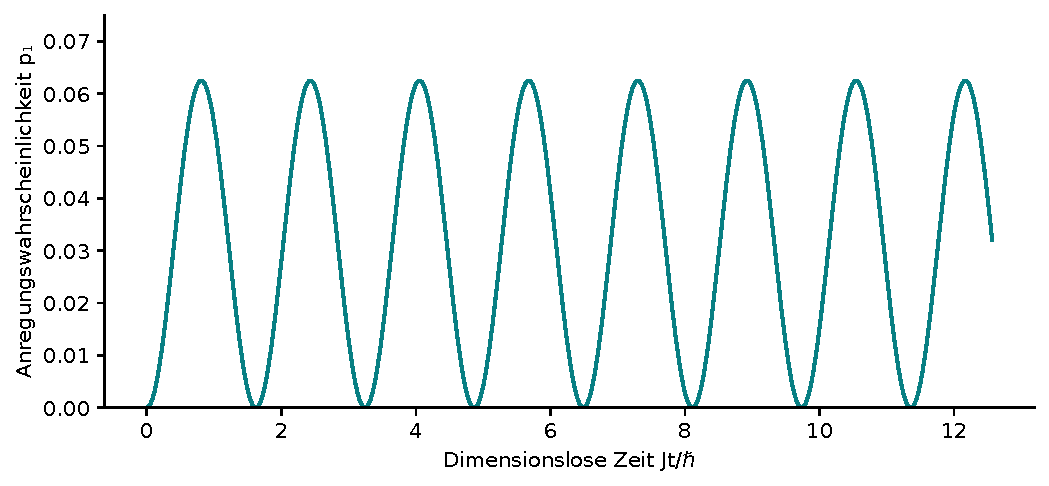
\includegraphics[width=.9\linewidth]{figures/two_cell_clock.pdf}
\caption{Das Zweizellensignal bei $\lambda=J$ und Produktanfangszustand. Seine kleine Amplitude ist Teil der Vorhersage. Der stationäre Grundzustand würde dieses Signal nicht zeigen.}
\end{figure}

Das ist autonome Bewegung unter einem gegebenen $H$, jedoch keine Ableitung einer äußeren Zeit oder von Sekunden. Es ist auch keine Vieranzeigenuhr und nicht der Familienzyklus mit Periode drei. Wiederholte Messungen und ihre gespeicherten Ergebnisse verlangen einen zusätzlichen, ausdrücklich einbezogenen Registerprozess.

\section{Warum viele Zellen noch ein eigener Schritt sind}
Ein einzelner eindeutiger Singulettgrundraum besitzt keine logische Zustandsvielfalt. Das Produkt solcher Grundräume bleibt eindimensional. Wer alles auf diese Grundräume projiziert, erhält nur eine skalare Energie. Nichttriviale effektive Dynamik muss Anregungen, Randzustände, Multiplizitäten oder zusätzliche Vakuumsektoren behalten.

Für $N$ vollständige Zellen mit $N-1$ positiven Brücken liefert der Produktzustand
\begin{equation}
E_0\le(N-1)\frac{5\lambda}{8},\quad
\Delta\ge2J-(N-1)\frac{5\lambda}{8}.
\end{equation}
Die einfache Eindeutigkeitsgarantie $\lambda<16J/[5(N-1)]$ verschlechtert sich mit der Zellzahl. Sie beweist keinen thermodynamischen Gap. Zudem kann ein zusammenhängendes Netz von mehr als vier Trägern nicht sämtliche Paarbedingungen mit Nullenergie erfüllen. Diese Frustration ist ein struktureller Befund und muss in jedem skalierenden Modell berücksichtigt werden.
